\chapter{Event Reconstruction
\label{ch:reconstruction}}

Particles created in proton-proton collisions pass through the CMS detector and leave signals in different subdetectors. Figure \ref{fig:cms-slice} shows examples of typical signals for different types of particles. Each type of particle has a different characteristic signature from which it can be identified using information from the various subdetectors. Muons, electrons, and charged hadrons create tracks in the tracker, while photons and neutral hadrons do not. Muons also create hits in the muon systems. Electrons and photons deposit energy in the ECAL, while charged and neutral hadrons deposit most of their energy in the HCAL. Neutrinos do not deposit any energy in the detector. Their presence must be inferred from missing transverse momentum, defined as the negative vector sum of \vecpt for all particles in the event: $\vecmet = - \sum_{i} \vecpt^{(i)}$. The magnitude of this quantity is called the missing transverse energy, denoted as \met. Because the incident proton beams have momentum only in the $z$ direction, any imbalance of measured momentum in the tranverse plane indicates particles which were not detected.

\begin{figure}[hbt]
\begin{center}
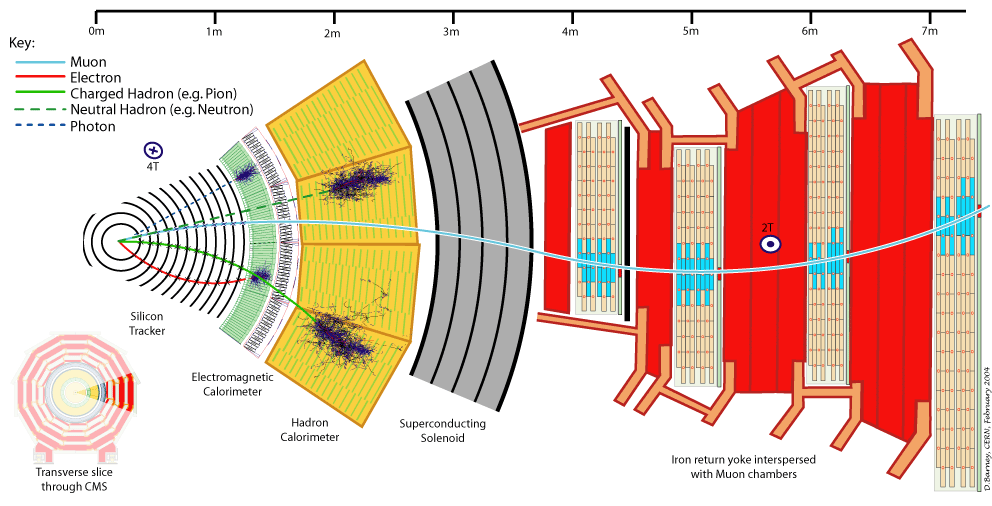
\includegraphics[width=0.95\textwidth]{figures/CMS_slice.png}
\caption{A cross-sectional view of the CMS detector with all subdetectors labeled and examples of signals left by muons, electrons, charged hadrons, neutral hadrons, and photons \cite{CMS-slice}.}
\label{fig:cms-slice}
\end{center}
\end{figure}

The raw output from each subdetector is processed in several steps in order to reconstruct the different types of particles \cite{TDR-software}. The first step is local reconstruction, which involves the creation of reconstructed hits or ``RecHits'' for each subsystem of each subdetector. The tracker RecHits include information about the positions of signals in the form of clusters, which are combinations of contiguous strips or pixels. The muon system RecHits also provide the positions of signals. In the DT and CSC subsystems, these RecHits can be combined into three-dimensional track segments. The ECAL and HCAL RecHits contain the energy, position, and time of energy deposits from traversing particles.

In the second step, global reconstruction, the RecHits from the different subsystems of a given subdetector are combined and further processed. In the tracker, pattern recognition algorithms are employed to reconstruct tracks for various cases, including displaced vertices, low \pt tracks, and high \pt tracks. The ECAL and HCAL RecHits are combined into calorimeter towers or ``CaloTowers'' using a projective $\eta$-$\phi$ geometry. ``Standalone'' muons are created by the muon system global reconstruction, which associates RecHits and track segments in a radial trajectory, accounting for bending by the residual magnetic field, and uses a vertex-constrained fit.

High-level reconstruction is the final step, in which information from all subdetectors is used to reconstruct various types of particles as precisely as possible. The particle types used in this search include electrons, muons, taus, jets, and b-jets. The reconstruction algorithms for these particles will be described in more detail in the following sections of this chapter. Many of these algorithms use a particle flow technique that is unique to CMS and will be described in Sec. \ref{sec:particle-flow}.

The CMS experiment uses detailed simulations to predict the performance of the detector and reconstruction algorithms and to model various physics processes. Each simulated event is generated from the interaction of partons in proton-proton collisions and the decays of the resulting particles, based on theoretical calculations. The traversal of the final state particles through the CMS detector is simulated, and after some processing, the results can be treated identically to the raw data from real events and used as input for the reconstruction software.

\section{Event Generation}

Protons are most basically considered to be composed of two up quarks and one down quark. However, as a QCD bound state, it is more accurate to consider those three quarks as valence quarks, the most prominent features in a quark-gluon sea of virtual particles. At high energies such as those present in LHC collisions, the presence of additional quarks and gluons, collectively called partons, becomes significant. The fraction of the momentum of a proton $A$ carried by a parton $a$ is defined as $x_a$, and the parton distribution function (PDF) for that parton is $f_{a/A}(x_a,Q^2)$, where $Q^2$ is the momentum scale of the interaction, typically the square of the total four-momentum in a collision. PDFs are calculated using experimental data sets, with different groups taking different approaches to analyzing the data and modeling proton behavior. The CMS experiment primarily uses PDFs from Martin-Stirling-Thorne-Watt (MSTW) and the Coordinated Theoretical-Experimental Project on QCD (CTEQ). Figure \ref{fig:pdf-mstw} shows an example set of PDFs calculated at NLO by MSTW \cite{MSTW09}. At high momentum scales, even bottom quarks may be present in the quark-gluon sea of a proton. The dependence of the PDFs on $Q^2$ is given by the Dokshitzer-Gribov-Lipatov-Altarelli-Parisi (DGLAP) equations \cite{QuarkGluon}.

\begin{figure}[hbt]
\begin{center}
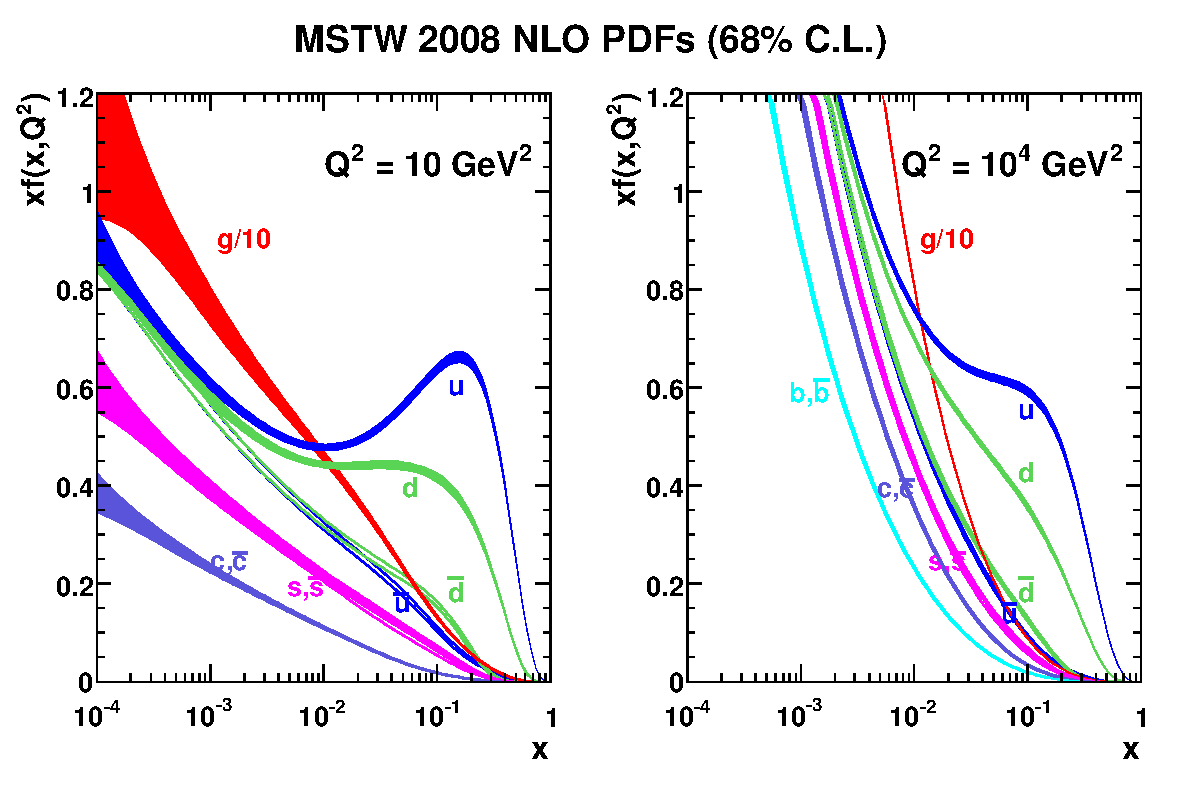
\includegraphics[width=0.95\textwidth]{figures/mstw2008nlo68cl_allpdfs.pdf}
\caption{PDFs calculated at NLO by MSTW, plotted against momentum fraction $x$ for two different values of the momentum scale $Q^2$ \cite{MSTW09}.}
\label{fig:pdf-mstw}
\end{center}
\end{figure}

The DGLAP equations allow large logarithmic factors, for example from col\-lin\-ear emission of gluons, to be included in the definition of the PDFs. This statement is the QCD factorization theorem, which applies to all hard-scattering processes. With this theorem, the interaction of parton $a$ in proton $A$ with parton $b$ in proton $B$, producing the final state $X$, can be written simply:
\begin{equation} \label{eq:hard-scatter}
\sigma_{AB \rightarrow X}(s) = \int{\text{dx}_{a}\text{dx}_{b} f_{a/A}(x_a,\mu_{F}^{2}) f_{b/A}(x_b,\mu_{F}^{2}) \hat{\sigma}_{ab \rightarrow X}(\hat{s},\mu_{R}^{2})}
\end{equation}
For such an interaction at high energy, the center-of-mass energy is $\sqrt{\hat{s}} = \sqrt{x_a x_b s}$, where $\sqrt{s}$ is the center-of-mass energy of the proton-proton system. There are two scales in Eq. \ref{eq:hard-scatter}: the factorization scale $\mu_{F}$ which separates long-distance physics from short-distance physics, and the renormalization scale $\mu_{R}$ of the QCD running coupling. Values for these scales are typically chosen to be characteristic of the hard scattering, with $\mu_{F} = \mu_{R}$. In addition to the primary hard-scattering process, the incoming protons and outgoing final state particles may radiate photons and gluons in processes called, respectively, initial state radiation (ISR) and final state radiation (FSR). The remnant partons which did not participate in the primary hard scatter may undergo soft interactions; these are collectively considered to be the ``underlying event''. All of these possible interactions in a proton-proton collision are visualized in Fig. \ref{fig:pp-collision}.

\begin{figure}[hbt]
\begin{center}
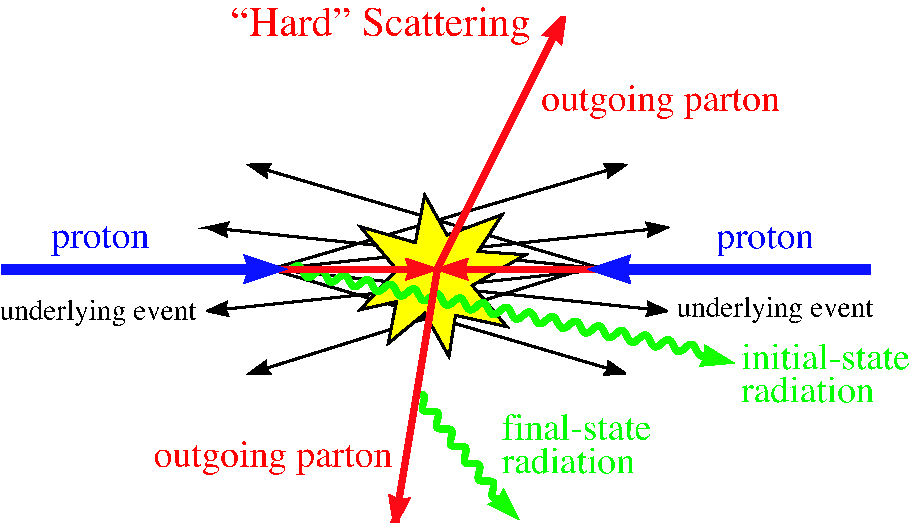
\includegraphics[width=0.95\textwidth]{figures/pp_collision_schematic.pdf}
\caption{An illustration of a proton-proton collision, showing the hard scattering, ISR, FSR, and the underlying event \cite{QuarkGluon}.}
\label{fig:pp-collision}
\end{center}
\end{figure}

Various event generation programs exist to simulate proton-proton collisions. The simulation of the hard scattering relies on a $2\rightarrow2$ matrix element to calculate $\hat{\sigma}_{ab \rightarrow X}(\hat{s},\mu_{R}^{2})$. Usually, the LO matrix element and PDFs are used for the simulation, and the results are scaled to NLO or NNLO using a $K$-factor derived from the ratio of the relevant cross sections. The program \PYTHIA \cite{Sjostrand:2006za} uses a parton showering approach to model ISR and FSR. Other generators such as \MADGRAPH \cite{MadGraph} use alternate approaches which more accurately simulate additional hard radiation outside of the primary hard scattering process, but must be combined with a program like \PYTHIA for showering from soft and collinear radiation. \POWHEG \cite{Alioli:2010xd} is a generator which uses NLO matrix elements and PDFs by matching them with parton shower contributions to prevent double counting. After the initial event generation, \MADGRAPH and \POWHEG are interfaced with \PYTHIA for hadronization. In addition, a specialized program called \TAUOLA \cite{TAUOLA} can be applied for accurate handling of tau lepton decays.

\section{Detector Simulation}

The response of the CMS detector to a proton-proton collision event is simulated using the stable final state particles output by event generators. The progression of each particle through the detector is tracked using the \GEANTfour software \cite{geant4nim,geant4ieee}. The geometry of every subdetector and subsystem is carefully simulated to ensure the accuracy of the simulation. The conditions of the real detector, including alignment and calibration changes, are measured periodically and stored in a database which can be used to configure the simulation. \GEANTfour includes customizable physics lists containing models of various physical processes to simulate the interactions of particles with matter. The detector simulation creates simulated hits or ``SimHits'' for each subdetector from the deposition of energy or charge based on those interactions. The effects of photodetectors and readout electronics on these SimHits are then simulated, mimicing the real subdetectors' data acquisition processes.

\section{Tracks and Vertices
\label{sec:tracks}}

Hits from the different tracker subsystems are reconstructed into charged-particle tracks using the Combinatorial Track Finder (CTF) algorithm \cite{TrackingJINST}. CTF is an iterative algorithm which finds the easiest tracks first, in order to remove the associated hits from consideration. This reduces the complexity of finding more difficult tracks in subsequent iterations. Each iteration follows the same four-step procedure, varying the type of seed used and the selection criteria applied.
\begin{enumerate}
\item A seed is generated using only a few hits.
\item Additional hits are added to the track based on the extrapolated trajectory of the seed.
\item The parameters of the track are estimated using a fit which considers all hits in the trajectory.
\item Selection criteria are applied to determine the quality of the track, and tracks which do not pass the selection are excluded.
\end{enumerate}

The types of seeds are categorized based on the number of hits included and the source of those hits. Initial iterations use pixel triplet and pair seeds, created from three and two pixel hits, respectively. These are the highest-quality seeds and are used to reconstruct prompt tracks, those emitting from primary vertices near the IP. A subsequent iteration uses a mixed triplet seed, containing 1--3 pixel hits and ${<}3$ strip hits. This iteration typically finds displaced tracks from heavy flavor decays, nuclear interactions, and photons which convert to \EpEm\xspace pairs in the tracker. The final iterations use strip pair seeds, consisting of two matched hits from the strip detectors, usually generated by charged particles which did not enter the pixel detector.

The iterations that use seeds with strip hits may also find prompt tracks which lack pixel hits. The specific sequence of iterations has been modified several times to improve the computing and physics performance of CMS tracking \cite{Tracking2012}. Table \ref{tab:tracking} lists the sequence used during the 2012 run. The selection criteria for each iteration are given, including cuts on \pt, transverse impact parameter $d_0$, and longitudinal impact parameter $z_0$. Some of the $z_0$ cuts are in terms of $\sigma$, the length of the beam spot in the $z$-direction used as a Gaussian standard deviation.

\begin{table}[htb]
  \begin{center}
    \begin{tabular}{llllll}
\hline
step  & seed type & seed subdetectors & \pt $[\GeVcns]$ & $d_0$ [cm] & $|z_0|$ \\
\hline
0     & triplet   & pixel             & ${>}0.6$     & ${<}0.02$  & ${<}4.0\sigma$ \\
1     & triplet   & pixel             & ${>}0.2$     & ${<}0.02$  & ${<}4.0\sigma$ \\
2     & pair      & pixel             & ${>}0.6$     & ${<}0.015$ & ${<}0.09\cm$ \\
3     & triplet   & pixel             & ${>}0.3$     & ${<}1.5$   & ${<}2.5\sigma$ \\
4     & triplet   & pixel/TIB/TID/TEC & ${>}0.5$--0.6 & ${<}1.5$   & ${<}10.0\cm$ \\
5     & pair      & TIB/TID/TEC       & ${>}0.6$     & ${<}2.0$   & ${<}10.0\cm$ \\
6     & pair      & TOB/TEC           & ${>}0.6$     & ${<}2.0$   & ${<}30.0\cm$ \\
\hline
    \end{tabular}
    \caption{The sequence of tracking iterations used during the 2012 run, including information on the seeds and selection criteria used in each step \cite{Tracking2012}.}
    \label{tab:tracking}
  \end{center}
\end{table}

The reconstructed tracks are used to reconstruct the primary vertices from the event \cite{TrackingJINST}. This includes both the main hard scatter vertex and additional vertices from pileup collisions. First, selection requirements are imposed on the tracks, in order to consider only prompt tracks near the IP. The selection requirements include cuts on the significance of $d_0$, the number of pixel and strip hits in the track, and the normalized $\chi^2$ from the fit of the track trajectory. The tracks which pass the selection requirements are clustered together using their $z$-coordinates, determined at each track's closest approach to the beam spot. A deterministic annealing algorithm is used to perform this clustering, in which each track may have a different probability to be associated with each vertex. The algorithm uses analogues of statistical mechanics quantities, slowly reducing the ``temperature'' and minimizing the ``free energy'' during each temperature iteration.

Once the deterministic annealing algorithm produces a list of vertex candidates, an adaptive vertex fitter is applied to each vertex candidate. This fitter weights each track in the vertex based on the agreement between the track and vertex positions. Using those weights, it fits the parameters of the vertex, including the $(x,y,z)$ position, the covariance matrix, and the number of degrees of freedom, $n_{\text{dof}} = -3 + 2 \sum{w_i}$, where $w_i$ is the weight for the $i$th track. The variable $n_{\text{dof}}$ can be used to select vertices which correspond to actual proton-proton interactions, as it is closely related to the number of tracks compatible with the vertex.

%add 2012 performance (efficiency, fake rate, vtx resolution)? references only have 2011 performance...

\section{Particle Flow
\label{sec:particle-flow}}

The CMS experiment uses a technique called particle flow (PF) to combine information from all subdetectors in order to identify all stable particles in each event \cite{CMS-PAS-PFT-09-001}. As described at the beginning of this chapter and shown in Fig. \ref{fig:cms-slice}, each type of stable particle is expected to create signals in a certain subset of the subdetectors. The performance of the PF algorithm was validated using early CMS data \cite{CMS-PAS-PFT-10-002,CMS-PAS-PFT-10-003}, along with newer CMS data for more recent uses of the algorithm \cite{Beaudette:2014cea}, demonstrating significant improvement over simpler approaches. The reconstructed particles are known as PF candidates, which can be treated as input particles by the various high-level reconstruction algorithms. PF candidates can also be used to compute the isolation of a reconstructed object, by summing the energy of candidates topologically close to the selected object.

The RecHits from the local reconstruction process are used to create the basic elements for this technique: tracks and clusters. Charged-particle tracks are created from tracker RecHits using an iterative algorithm as described in Sec. \ref{sec:tracks}, and muon tracks are created from muon system RecHits. Calorimeter energy deposits are grouped into clusters by identifying seed hits as local energy maxima exceeding a certain threshold, and then adding neighboring hits with energy above subsystem-specific thresholds meant to eliminate photodetector noise. Further removal of noise from the calorimeters is performed by rejecting clusters with characteristics matching those expected from leading sources of noise. Tracks and clusters are associated together using a linking algorithm that determines if they were likely produced by the same particle. The algorithm considers a possible link between each algorithm based on the $\eta$-$\phi$ distance between a charged-particle track and a cluster, accounting for propagation in the magnetic field, or between two clusters. For links between a charged-particle track and a muon track, the $\chi^{2}$ value from a global fit is used as the link distance. Groups of elements are associated based on minimizing the link distance and are called ``blocks''.

PF reconstruction algorithms classify the blocks as different types of particles. When a block is classified as a certain type of particle, it is removed from the list of unclassified blocks. A global muon block is accepted as a PF muon if the momentum of the combined charged-particle and muon tracks agrees with the momentum of the charged-particle track alone. The energy expected to have been deposited by the PF muons in the calorimeters due to minimum ionization is subtracted from the clusters. The remaining charged-particle tracks are checked for compatibility with electrons, which tend to leave short tracks and radiate energy via bremsstrahlung. A Gaussian Sum Filter (GSF) is applied to the compatible tracks in order to identify spatially-matched ECAL clusters, and the combination of a track and one or more clusters is classified as a PF electron.

The remaining tracks are linked to clusters to form PF charged hadrons, if the total cluster energy is similar to but smaller than the total track momentum. More than one track can link to a given cluster, but for a given track, only the link to the closest cluster is kept. This reflects the coarser segmentation of the calorimeter system as compared to that of the tracker. In cases where the total cluster energy is significantly smaller than the total track momentum, additional PF muons may be found using tracks from the block, and some tracks may be classified as fake and removed from consideration. Finally, an excess of energy in the clusters, above the total track momentum, is assumed to come from neutral particles. The excess energy is typically classified as a PF photon. If the total excess cluster energy in a block is larger than the total ECAL energy in the cluster, a PF neutral hadron is created from the excess energy remaining after assigning the ECAL excess energy to a PF photon. The remaining clusters not linked to any tracks are used to create PF photons in ECAL and PF neutral hadrons in HCAL.

\section{Electrons
\label{sec:ele-reco}}

The electron candidates reconstructed by the PF algorithm are considered to be ``tracker-driven'' \cite{CMS-PAS-EGM-10-004}. This approach is suitable for low-\pt electrons and electrons produced by jets. For higher-\pt electrons, an alternative ``ECAL-driven'' approach is used. ECAL clusters are grouped into superclusters to account for bremsstrahlung photons radiated by electrons as they traverse the tracker, as well as the spread of energy in the $\phi$-direction due to the magnetic field \cite{ElectronReco}. Similarly to the PF algorithm, these superclusters are matched with track seeds and a GSF is used to reconstruct the trajectory of the electron track. Using a mixture of Gaussians to select the electron track better accounts for the energy loss from bremsstrahlung, as compared to the standard CMS track finding procedure \cite{ElectronGSF}. The lists of tracker-driven and ECAL-driven electron candidates are compared to avoid double counting.

Quality cuts on various kinematic variables are applied to the GSF electron candidates to identify whether or not they are genuine electrons \cite{ElectronCutBased}. A set of cut values is called a working point, and multiple working points are defined based on the strictness of the cut values. The kinematic variables used in the quality cuts are described here, and the specific values of the quality cuts used in the dissertation will be listed in Sec. \ref{sec:ele-obj}. The $\eta$ width of the supercluster, $\sigma_{i\eta i\eta}$, is taken from the covariance matrix of the $\eta$ positions of the included crystals compared to the seed cluster. A modified $\eta$ variable which accounts for the crystal spacing is used, and each crystal's contribution is weighted using the logarithm of the ratio of its energy to the seed cluster energy \cite{EgammaShowerShape}. The differences in position of the supercluster, $(\eta_{\text{sc}},\phi_{\text{sc}})$, and the extrapolated track, $(\eta_{\text{in}}^{\text{extrap}},\phi_{\text{in}}^{\text{extrap}})$, are defined as $|\Delta \eta_{\text{in}}| = |\eta_{\text{sc}} - \eta_{\text{in}}^{\text{extrap}}|$ and $|\Delta \phi_{\text{in}}| = |\phi_{\text{sc}} - \phi_{\text{in}}^{\text{extrap}}|$. The leakage energy $H$ in the HCAL tower located behind the ECAL seed cluster is compared to the energy of the seed cluster $E$ in the variable $H/E$. The transverse and longitudinal impact parameters of the vertex associated with the electron, $d_{0}^{\text{vtx}}$ and $z_{0}^{\text{vtx}}$, are used. The variable $|1/E - 1/p|$, comparing the electron energy and momentum, is also considered. Finally, the isolation is computed by summing the \pt of charged hadron (CH), neutral hadron (NH), and photon ($\gamma$) PF candidates within a cone of $\Delta R < 0.3$ of the electron candidate, including a correction for contributions from pileup based on the median energy per area $\rho$ and the effective area of the electron $A_{\text{eff}}$:
\begin{equation}
I^{\text{PF}}_{\Pe} = \sum_{\Delta R < 0.3}{\pt^{(\text{CH})}} + \text{max}\left( \sum_{\Delta R < 0.3}{\pt^{(\text{NH})}} + \sum_{\Delta R < 0.3}{\pt^{(\gamma)}} - \rho A_{\text{eff}}, 0 \right).
\end{equation}
The relative isolation $I^{\text{PF}}_{\Pe}/\pt^{(\Pe)}$, scaled by the \pt of the electron, is used for the quality cuts.

\section{Muons
\label{sec:muon-reco}}

The PF muon candidates are used for muon reconstruction. In addition, two supplementary methods are used to reconstruct muons \cite{CMS-PAS-MUO-10-002}. The first method considers all charged-particle tracks from the tracker, above minimal \pt and $p$ cuts, and creates a tracker muon from any track whose extrapolated position matches a track segment in the muon system. This method is efficient for low-momentum muons. The second method produces global muons. This method starts with a standalone muon from a track segment in the muon system and finds a matching track from the tracker. A global muon fit is then performed using both the muon system and tracker tracks, which can provide better momentum resolution for high-\pt muons. The global and track muon candidates, along with any remaining standalone muons which were not matched to a charged-particle track, are combined into one collection in order to prevent double counting.

As with electrons, working points are defined based on sets of quality cuts with different strictness. These cuts can include minimum numbers of muon system hits and segments, as well as minimum numbers of pixel hits and overall tracker hits. The reduced $\chi^2$ from the global muon fit is considered. The distances between the primary vertex and the transverse and longitudinal impact parameters $d_0$ and $d_z$ of the tracker track are also used. The isolation is calculated using PF candidates within a cone of $\Delta R < 0.4$ of the muon:
\begin{equation}
I^{\text{PF}}_{\mu} = \sum_{\Delta R < 0.4}{\pt^{(\text{CH})}} + \text{max}\left( \sum_{\Delta R < 0.4}{\pt^{(\text{NH})}} + \sum_{\Delta R < 0.4}{\pt^{(\gamma)}} - \Delta\beta \sum_{\Delta R < 0.4}{\pt^{(\text{PU})}}, 0 \right).
\end{equation}
A $\Delta\beta$ pileup (PU) correction is applied using the \pt of PU particles, which are identified as charged PF candidates from a different vertex than the muon. The $\Delta\beta$ factor is assigned a value of 0.5 based on the expected ratio of charged to neutral particles in pileup \cite{CMS-PAS-PFT-10-002}. Again, cuts are made on the relative isolation $I^{\text{PF}}_{\mu}/\pt^{(\mu)}$. The selections on these quantities are intended to minimize the contribution from cosmic ray muons, muons from heavy flavor decays, and leakage from hadronic showers. They also ensure precise measurement of the muon \pt. Section \ref{sec:muon-obj} will provide the specific cuts for the working points used in the dissertation.

\section{Jets}

Due to QCD confinement, strongly interacting particles, quarks and gluons, cannot exist in a bare state. They immediately form multiple color singlet bound states, hadrons, using the energy from the gluon field in a process called hadronization. These hadrons tend to be produced in a narrow spray, which is called a jet \cite{Salam:2009jx}. To reconstruct a jet, the component particles must be clustered together. CMS uses the anti-\kt algorithm \cite{Cacciari:2008gp} to perform this clustering. This algorithm is a specific case of a generalized iterative cone algorithm, using the following equations:
\begin{align}
d_{ij} &= \text{min}(p_{\text{T}i}^{2p},p_{\text{T}j}^{2p})\frac{\Delta R_{ij}^{2}}{R^{2}}, \\
\Delta R_{ij}^{2} &= (\eta_i - \eta_j)^2 + (\phi_i - \phi_j)^{2}, \\
d_{iB} &= p_{\text{T}i}^{2p}.
\end{align}
Two distance variables are defined: the distance between particles $i$ and $j$, $d_{ij}$, and the distance between particle $i$ and the beam, $d_{iB}$. These distances are weighted by the \pt of the particles as indicated, and $R$ is a size parameter. At each iteration, both distance variables are calculated for all particles. If the minimum distance is $d_{iB}$, particle $i$ is considered to be a fully-clustered jet and removed from the list of particles. Otherwise, particles $i$ and $j$ from the minimum $d_{ij}$ are grouped together in the particle list. The algorithm continues to iterate until the particle list is empty. The anti-\kt algorithm is a special case of these equations with parameter $p=-1$. It has many desirable properties, including infrared and collinear safety, and the creation of circular jets with radius $R$ as shown in Fig. \ref{fig:ak5-example}.

\begin{figure}[hbt]
\begin{center}
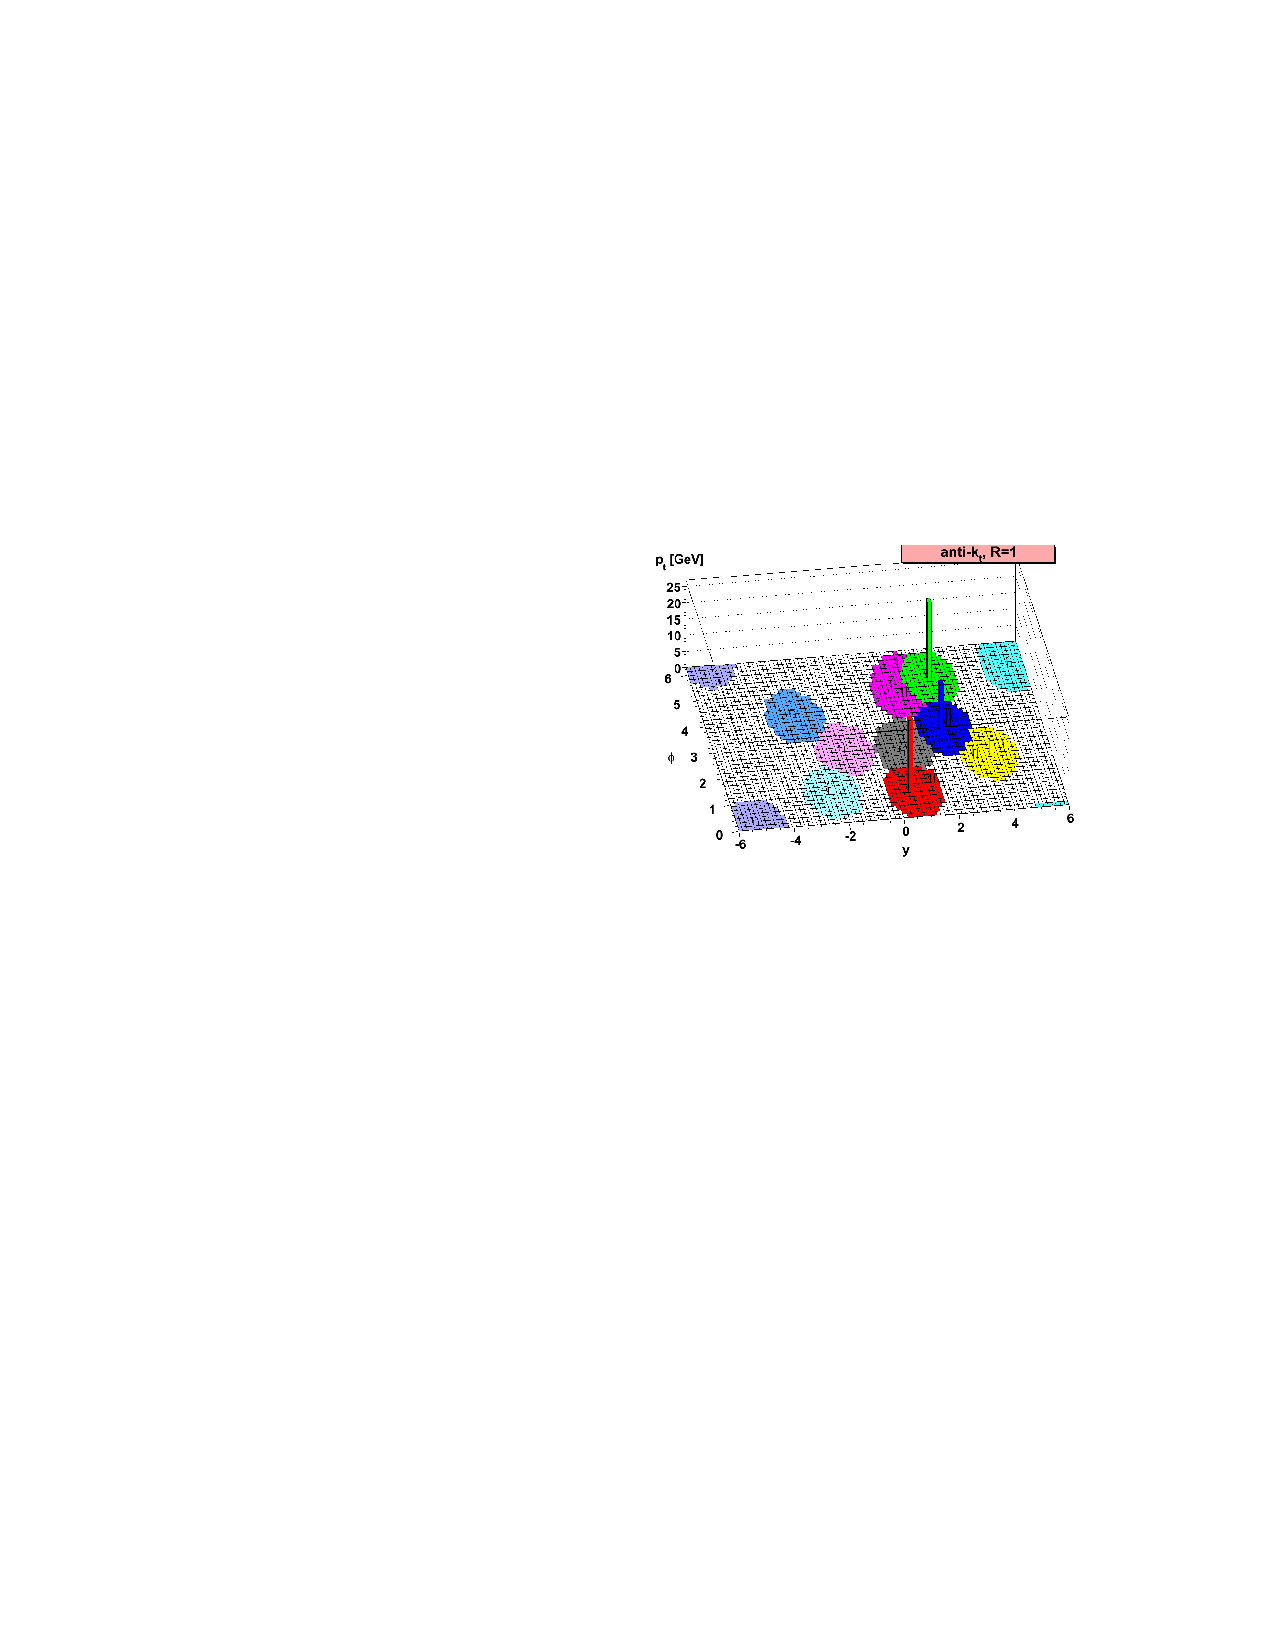
\includegraphics[width=0.95\textwidth]{figures/08021189v2-fig.pdf}
\caption{An example of jets reconstructed with the anti-\kt algorithm, demonstrating the characteristic circular shape \cite{Cacciari:2008gp}.}
\label{fig:ak5-example}
\end{center}
\end{figure}

CMS chooses the value $R = 0.5$ for the size parameter and uses PF candidates for clustering, producing PF jets \cite{CMS-PAS-PFT-09-001, CMS-PAS-PFT-10-002}. Alternative jet methods use CaloTowers and charged-particle tracks separately or together, but these do not perform as well as PF jets. Typically, 65\% of jet energy goes into charged particles, 25\% goes into photons, and 10\% goes into neutral hadrons. Using PF candidates takes advantage of the excellent energy and position resolution for charged particles and photons provided by the combination of the tracker and the calorimeters in the PF algorithm.

Once a jet is reconstructed, several important types of corrections are applied to its energy response \cite{CMS-JEC}. First, minimum bias events are used to estimate the contributions from electronic noise and pileup, and those are subtracted in the offset correction. Next, the energy response is made uniform in $\eta$ using the multiplicative relative correction, derived from dijet events. Finally, the multiplicative absolute correction is derived from \GZJ events, exploiting the precise energy resolution of the ECAL and the tracker, and applied to make the energy response uniform in \pt.

To ensure the quality of reconstructed jets used in data analysis, a set of variables is used for PF jet identification \cite{CMS-AN-2010-003}. These variables include: the fraction of neutral hadrons in the jet, the fraction of neutral EM particles, the fraction of charged hadrons, the fraction of charged EM particles, the number of constituents, and the multiplicity of charged particles. Multiple sets of cuts on these variables are defined as working points \cite{PFJetID}. The specific working point used in this dissertation will be given in Sec. \ref{sec:jet-obj}.

\section{Taus
\label{sec:hpstau}}

Tau leptons decay into hadrons approximately 64.76\% of the time \cite{PDG}. These hadronic decays produce objects similar to jets, but typically narrower and more isolated. For this reason, PF jets are used as the basis for reconstructing hadronically decaying tau leptons (hadronic taus or $\tauh$s). The Hadron Plus Strips (HPS) algorithm is used to identify tau leptons \cite{TauPerfCMS,Calabria:1516071}. The vast majority of \tauh decays consist of a tau neutrino $\nu_{\tau}$, one or three charged hadrons $h^{-}$ that are either $\pi^{-}$ or $K^{-}$, and zero or more neutral hadrons $\pi^{0}$ that almost immediately decay to two photons. The HPS algorithm only considers the visible decay products, so the $\nu_{\tau}$ is ignored. Table \ref{tab:tauh-decay} lists the leading hadronic decays, including intermediate hadronic resonances when present.

\begin{table}[htb]
  \begin{center}
    \begin{tabular}{|l|l|l|l|}
\hline
Decay                                                       & Resonance   & Mass (\MeVccns) & Branching fraction (\%) \\
\hline
$\tau^{-} \rightarrow h^{-} \nu_{\tau}$                     &             &                 & 11.53\% \\
$\tau^{-} \rightarrow h^{-} \pi^{0} \nu_{\tau}$             & $\rho^{-}$  & 775             & 25.95\% \\
$\tau^{-} \rightarrow h^{-} \pi^{0} \pi^{0} \nu_{\tau}$     & $a_{1}^{-}$ & 1230            & 9.52\% \\
$\tau^{-} \rightarrow h^{-} h^{+} h^{-} \nu_{\tau}$         & $a_{1}^{-}$ & 1230            & 9.80\% \\
$\tau^{-} \rightarrow h^{-} h^{+} h^{-} \pi^{0} \nu_{\tau}$ &             &                 & 4.76\% \\
\hline
    \end{tabular}
    \caption{The leading hadronic decays of tau leptons, including branching fractions and intermediate hadronic resonances \cite{PDG}. The symbol $h^{-}$ can be either $\pi^{-}$ or $K^{-}$. }
    \label{tab:tauh-decay}
  \end{center}
\end{table}

The strips in the HPS algorithm consist of PF photon candidates. Starting with the most energetic photon in the PF jet, the strip is built using an iterative search for other photons within a range $0.20\times0.05$ in $\eta$-$\phi$ around the center of the strip. Each iteration accepts the most energetic photon found and then recalculates the four-momentum of the updated strip. The strip is complete once no remaining photons are found in the given window, and it is kept if it passes a minimum \pt cut. The procedure is repeated with any remaining ungrouped photons in the jet. The formation of strips from photons accounts for spreading of their energy due to the effect of the magnetic field on conversions in the tracker.

Using the constituents of the PF jet, all combinations of strips with one or three charged hadrons are tested, with the charged hadrons assumed to be pions. All strips and charged hadrons must be found within a cone of $\Delta R = \text{max}(\text{min}(0.10,3.0/\pt^{\tauh}),0.05)$, where $\pt^{\tauh}$ is the \pt of the \tauh candidate in \GeVns. Several decay mode topologies are included in the algorithm, with mass ranges enforced for candidates based on the expectation of hadronic resonances in decays \cite{CMS-AN-2014-008}. Figure \ref{fig:tau-modes} shows a simple diagram of the different topologies.
\begin{enumerate}
\item Single hadron, when no strips are found.
\item One hadron + one strip, when the $\pi^0$ decay creates one strip from two narrowly separated photons. The invariant mass of the \tauh candidate, $M_{\tauh}$, must be in the range $0.3 < M_{\tauh} < \text{max}(1.3,\text{min}(1.3\sqrt{\pt^{\tauh}/200},2.1))\GeV$.
\item One hadron + two strips, when the $\pi^0$ decay creates one strip from two narrowly separated photons. In this case, the invariant mass of the two strips combined, $M_{\text{strips}}$, must be in the range $50 < M_{\text{strips}} < 200\MeV$, and $M_{\tauh}$ must be in the range $0.4 < M_{\tauh} < \text{max}(1.2,\text{min}(1.2\sqrt{\pt^{\tauh}/200},2.0))\GeV$.
\item Three hadrons, which requires all three charged hadron candidates to originate from the same primary vertex and to have the appropriate electric charges. $M_{\tauh}$ must be in the range $0.8 < M_{\tauh} < 1.5\GeV$.
\end{enumerate}
If more than one combination of PF constituents passes these decay mode finding requirements, the combination with the highest $\pt^{\tauh}$ is selected.

\begin{figure}[hbt]
\begin{center}
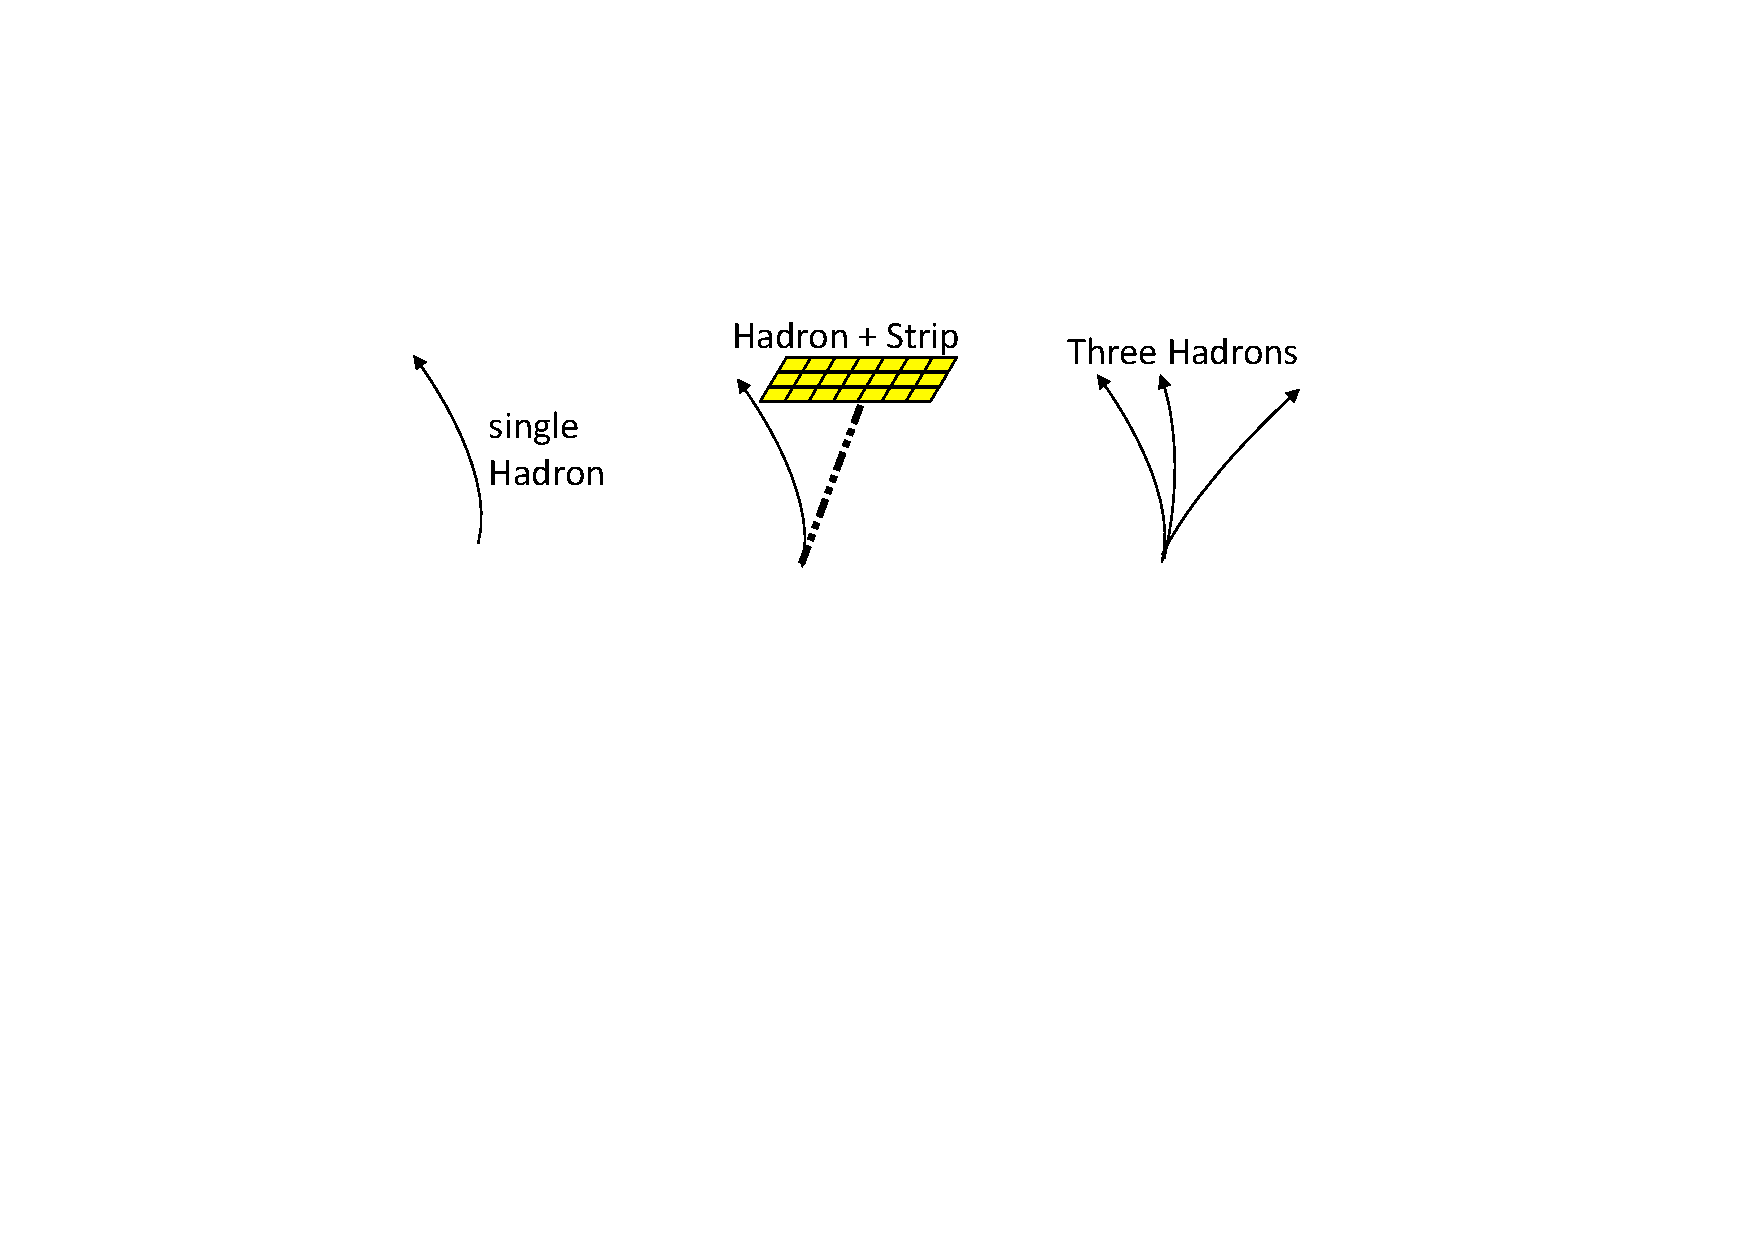
\includegraphics[width=0.95\textwidth]{figures/DP2014_015-fig.pdf}
\caption{A simple diagram of the different hadronic tau decay mode topologies reconstructed by the HPS algorithm \cite{CMS-DP-2014-015}.}
\label{fig:tau-modes}
\end{center}
\end{figure}

Isolation is an important tool in discriminating between $\tauh$s and jets. The isolation variable is computed using charged hadron and photon PF candidates within a cone of $\Delta R < 0.5$ around the \tauh candidate. A $\Delta\beta$ PU correction is applied using PU particles within a cone of $\Delta R < 0.8$ which originate from a different vertex than the \tauh candidate, with the factor $\Delta\beta = 0.4576$ \cite{CMS-DP-2014-015}.
\begin{equation}
I^{\text{PF}}_{\tauh} = \sum_{\Delta R < 0.5}{\pt^{(\text{CH})}} + \text{max}\left( \sum_{\Delta R < 0.5}{\pt^{(\gamma)}} - \Delta\beta \sum_{\Delta R < 0.8}{\pt^{(\text{PU})}}, 0 \right).
\end{equation}
The HPS algorithm uses the absolute isolation $I^{\text{PF}}_{\tauh}$ for the different working point quality cuts. The isolation discrimination also requires that each track associated with the \tauh contain at least three hits in the tracker. In addition to isolation, it is necessary to discriminate against electrons and muons which are misidentified as $\tauh$s. The anti-electron discriminator uses a multivariate (MVA) approach, training boosted decision trees (BDTs) using numerous variables depending on different cases of \tauh. These cases include: the possible association of the primary charged hadron in the \tauh with a GSF track; the possible association of the \tauh with a GSF electron within a cone of $\Delta R < 0.3$; whether or not the \tauh includes strips; and whether the \tauh $\eta$ coordinate lies in the EB or EE range. Multiple trainings for the anti-electron MVA discriminator were performed and multiple working points are defined. The anti-muon discriminator uses a cut-based approach, with multiple sets of cuts and working points defined. The cuts include requirements to minimize the activity in the muon system in the direction of the \tauh and to veto MIP muons based on energy and momentum. The specific working points for each discriminator used in this dissertation will be described in Sec. \ref{sec:tau-obj}.
%The \tauh candidate must not match any muon track segments or any hits in the two outermost muon stations within a cone of $\Delta R < 0.5$. In the single hadron decay mode, the charged hadron in the \tauh must have $(E_{\text{ECAL}} + E_{\text{ECAL}})/p_{\text{track}} > 0.2$.

\section{b-tagging
\label{sec:b-tagging}}

Bottom quarks are associated with many interesting physical signatures, including decays of top quarks and Higgs bosons, as well as many BSM theories, including supersymmetry, that privilege or otherwise relate to third-generation fermions. Jets generated by bottom quark hadronization, b-jets, can be identified using certain properties which set them apart from jets from lighter quarks or gluons \cite{BTV-12-001}. Bottom quarks form hadrons with relatively long lifetimes whose decay products tend to have high \pt. Numerous algorithms have been created to identify b-jets based on information from tracks or reconstructed secondary vertices from b-hadron decays. The most successful of these algorithms is the Combined Secondary Vertex (CSV) algorithm, which uses secondary vertices and adds information from the tracks. The CSV algorithm calculates a likelihood-based discriminator to separate b-jets and other jets. Loose, medium, and tight working points are defined for this discriminator, based on setting the probability of misidentifying a light quark or gluon jet as a b-jet to be 10\%, 1\%, and 0.1\%, respectively \cite{CMS-PAS-BTV-13-001}.

For a given jet, the CSV algorithm subjects the tracks within that jet to additional purity requirements, beyond those specified in Sec. \ref{sec:tracks}. The track must fall within a cone of $\Delta R < 0.3$ relative to the direction of the jet and the distance between the track and the jet at closest approach must be less than 0.07\cm. The track must include at least two pixel hits and at least eight total tracker hits, with $\chi^2/n_{\text{dof}} < 5$. The impact parameters between the track and the primary vertex must satisfy $d_0 < 0.2\cm$ and $d_z < 17\cm$. Finally, the track must have $\pt>1\GeVc$ and decay length less than 5\cm, where decay length is the distance between the primary vertex and the closest approach of the track and the jet. The significance of the track's impact parameter $S_{\text{ip}}$, defined as the value of the impact parameter divided by its uncertainty, is a powerful observable. The number of high-quality tracks in the jet is also used.

Secondary vertices are reconstructed using the adaptive vertex fitter, which was described in Sec. \ref{sec:tracks}. Candidates are rejected if ${\geq}65\%$ of their tracks are also associated with the primary vertex; if they are outside a cone $\Delta R < 0.5$ with respect to the jet direction; or if they are radially separated from the primary vertex by more than 2.5\cm with an invariant mass close to the $\cmsSymbolFace{K}^{0}$ mass. The CSV algorithm assigns jets into one of three categories based on the presence of a secondary vertex: real vertex, pseudo-vertex, and no vertex. In the pseudo-vertex case, the algorithm uses tracks with $S_{\text{ip}} > 2$ to create an effective secondary vertex when the adaptive vertex fitter fails. In the no vertex case, the algorithm defaults to use only the track-based variables described previously. Otherwise, the vertex variables used include:
\begin{itemize}
\item The significance of the flight distance between the secondary and primary vertices in the transverse plane.
\item The mass of the secondary vertex.
\item The number of tracks in the secondary vertex.
\item The ratio between the energy in the secondary vertex tracks and the energy in all the tracks in the jet.
\item The $\Delta\eta$ values between each the secondary vertex track and the jet.
\item The transverse impact parameter significance for the track that pushes the invariant mass of the secondary vertex above 1.5\GeVcc, the threshold for charm quarks. This is calculated by sorting the tracks by $S_{\text{ip}}$ and combining them one by one.
\end{itemize}